\chapter{Methodology}

This chapter contains a comprehensive description of the design of the proposed matching system, and demonstrates how its novel contributions address the ontology matching problem. Core reasoning steps and the use of code and APIs are introduced.

\section{Ontology Matching Workflow}

The general workflow of a typical ontology matching methodology is given in Figure \ref{fig:methodology1}. This explains how a matcher is used, as well as how they can be enhanced in an iterative manner.

\begin{figure}[ht]
\begin{center}
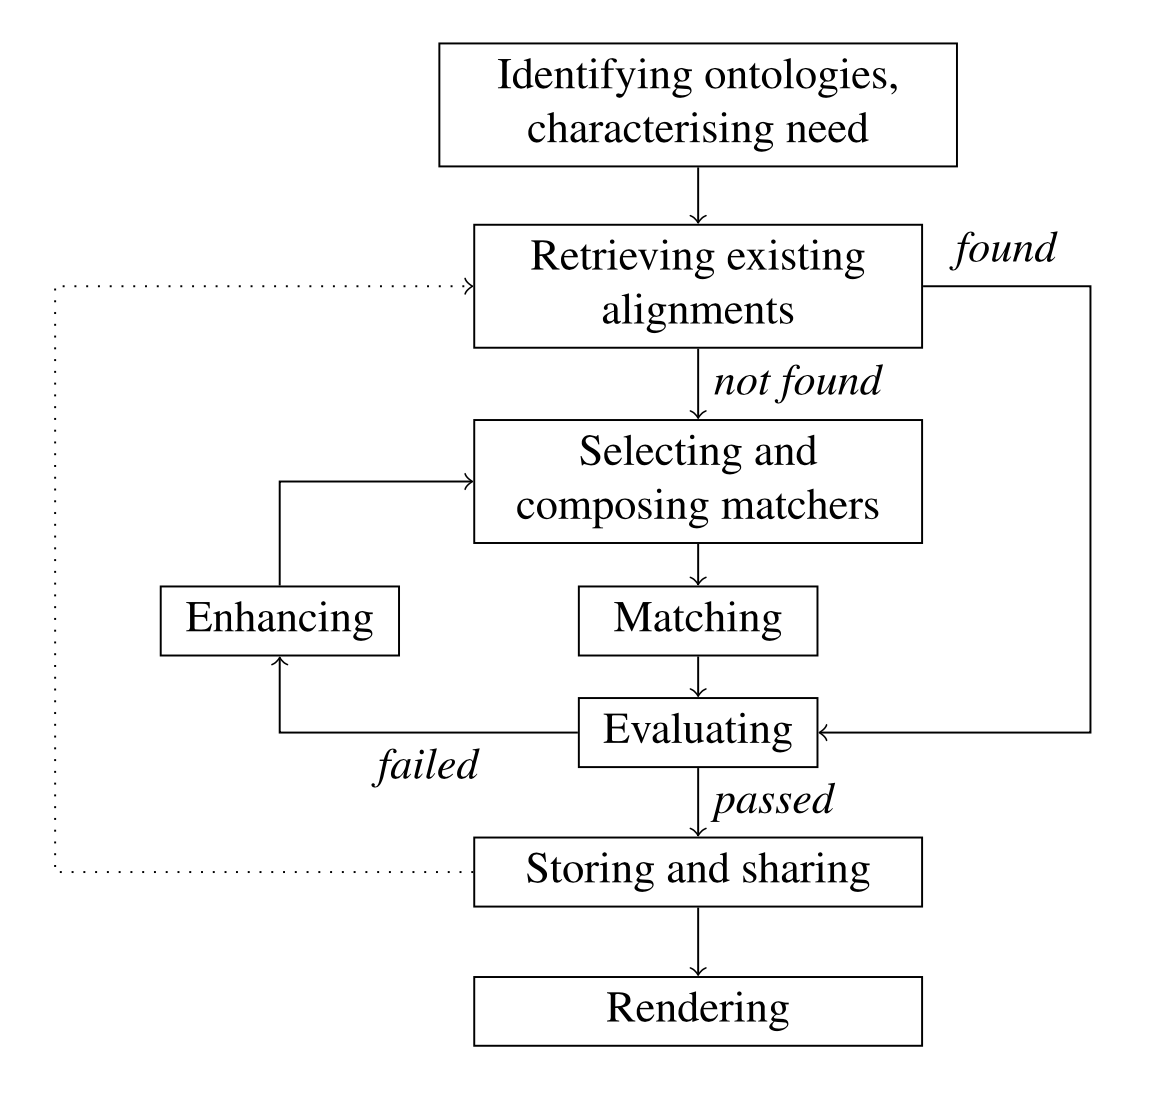
\includegraphics[width=0.4\textwidth]{img/methodology1.png}
\caption{The Ontology Matching Methodology}
\label{fig:methodology1}
\end{center}
\end{figure}

The process starts by identifying the need, or what kind of alignments are expected as the result of the matching. Then existing alignments between the input ontologies are retrieved from available resources or previous matching results as a basement. If the existing alignments does not satisfy the need, a matcher should be selected and composed to perform the matching, producing alignments results to be evaluated. The matcher enhances itself with the evaluation results iteratively until satisfying results are generated. The final alignment is then stored and shared as available resource, possibly rendered to different formats.

\section{Algorithm Design}

Based on the motivations explained in Section 1.2, this project seeks to improve the matching of instances with the help of extra information from ontologies and description logic reasoners. Therefore, when selecting the ontologies, it is best if they include high quality definitions of object properties, data properties and class relations, as well as sufficient amount of instances. Also, the reference alignment used for evaluation should include matching entities of different types, ideally classes, instances and even object and data properties. With that in mind, the ontology matcher should possess adequate reasoning capabilities to utilise those information. According to the structures of existing popular systems and the evaluation results provided in Section 2.2, the systems LogMap, Lily and PARIS, especially LogMap, are decided to be investigated into for several reasons. Lily has shown excellent performance in the SPIMBENCH instance matching tracks, with not only high precision, F-measure and recall rate, but also a reasonable time efficiency. However, it uses a fully similarity-based approach for identifying matching instances, utilising only Edit Distance of strings and similarity of structures, which does not constitute a solid foundation for reasoning. PARIS, being a probability-based system, deals with not only classes and instances, but also tries to align instance relations. It is worth investigating what kind of data structures PARIS implements to store those extra information. LogMap was designed to be able to deal with large-scaled ontologies for general purposes, which suits the need of matching enormous classes and instances in data integration. More importantly, it is largely based on logical reasoning and unsatisfiability repair, which can serve as a good foundation for reasoning with description logic reasoners. Therefore, based on the outstanding characteristics of their structures, especially the structure adopted by LogMap, the design of the matching system is proposed in Figure \ref{fig:Structure}.

\begin{figure}[ht]
\begin{center}
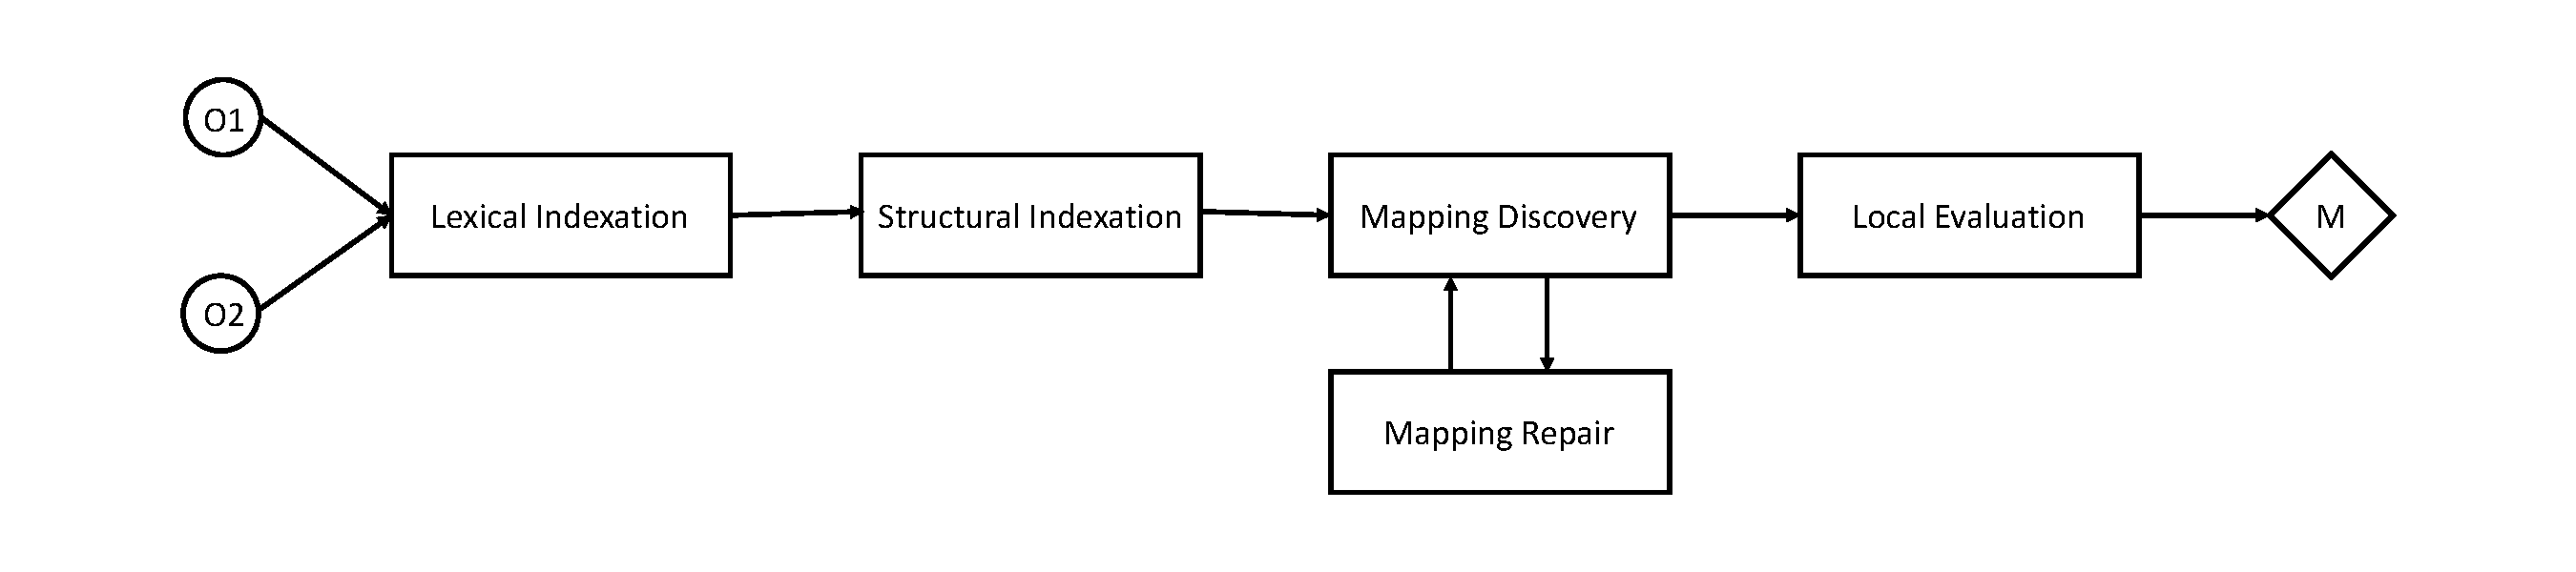
\includegraphics[width=\textwidth]{img/Structure.pdf}
\caption{System Design}
\label{fig:Structure}
\end{center}
\end{figure}

The methodological design of the system shows that the matching is performed in several stages. First, the axioms in the input ontologies $O1$ and $O2$, including not only classes and instances, but also object properties, data properties, annotations, datatypes and values, are read and parsed. Then, the labels for those entities are processed and put into a data structure called inverted index table \cite{DBLP:conf/semweb/Jimenez-RuizG11}. This makes it much easier to index the entities by individual lexicons in their labels. Table \ref{tab:INVERTED_TABLE} shows an example transformation from the original label to the inverted table.

\begin{table}[ht]
\centering
\resizebox{0.75\textwidth}{!}{%
\begin{tabular}{|l|l|l|l|}
\hline
\multicolumn{2}{|c|}{Original Label}                & \multicolumn{2}{c|}{Inverted Table}                  \\ \hline
\multicolumn{1}{|c|}{ID} & \multicolumn{1}{c|}{URI} & \multicolumn{1}{c|}{Entry} & \multicolumn{1}{c|}{ID} \\ \hline
1                        & DissertationSupervisor   & Dissertation, Supervisor   & 1                       \\ \hline
2                        & Module\_Dissertation     & Module, Dissertation       & 2                       \\ \hline
                         &                          & Dissertation               & 1, 2                    \\ \hline
                         &                          & Supervisor                 & 1                       \\ \hline
                         &                          & Module                     & 2                       \\ \hline
\end{tabular}%
}
\caption{Inverted Index Table}
\label{tab:INVERTED_TABLE}
\end{table}

Note how the labels are processed into lexicons first, with redundant string parts removed, and the lexicon ``Dissertation'' can now be used to index the entity IDs related to it, namely $1$ and $2$. This is followed by the structural indexation step, which computes the basic hierarchical relationships between the classes with the help of a description logic reasoner. For the completeness of reasoning, the fully fledged reasoner HermiT is used. This makes it possible to discover hierarchies hidden in complex axioms, and to utilise the role axioms for reasoning about classes, such as the ``DT and Modules'' example given in Section 1.2. However, it is worth mentioning that OWL 2 implements three profiles with different level of expressiveness, and using a profile-specific reasoner to target an ontology in a specific profile can reduce the reasoning time greatly. Therefore, in case the full systematic reasoning takes too long to compute for large ontologies, a basic structural reasoner is activated to replace HermiT as appropriate. The computed class hierarchies are stored in an Interval Labeling Schema \cite{DBLP:conf/semweb/Jimenez-RuizG11}, which is an optimised data structure for storing directed acyclic graphs (DAGs). It essentially uses integer intervals to keep track of the predecessors and descendants of a class. After that, the iterative process of mapping discovery and mapping repair starts, which is the core stage of this system. New mappings are discovered and repaired by description logic reasoning with all possible information at hand, including class assertions, instance assertions, role assertions, datatype and value assignments, and annotations. At the discovery stage, string distances between entities are calculated, and entities with high similarities are selected as candidates. The candidates are then processed by a description logic reasoner which intensively checks for unsatisfiability, eliminating inconsistencies and keeping the good matches as anchors. After reasoning about these new anchors with existing knowledge for further knowledge acquisition, the anchors are used as a starting set for mapping discovery in the next iteration. Tables \ref{tab:OWL_CLASS_CONSTRUCTOR} and \ref{tab:OWL_AXIOM} summarise the OWL class constructors and axioms that can be reasoned with the help of a description logic reasoner. In these tables, $C$ is a class, $x$ is an instance, $p$ is an object property, $d$ is a data property, $D$ is a datatype, and $v$ is a data value. The subscripts are non-negative integers. Although not all of these reasoning features are exploited, these can serve as a reference for future implementation.

\begin{table}[ht]
\centering
\resizebox{0.5\textwidth}{!}{%
\begin{tabular}{|l|l|}
\hline
\multicolumn{1}{|c|}{OWL Class Constructors} & \multicolumn{1}{c|}{Description Logic} \\ \hline
ObjectInverseOf($p$)                           & $p^-$                                     \\ \hline
ObjectPropertyChain($p_1$ ... $p_n$)             & $p_1 \circ ... \circ p_n$                          \\ \hline
ObjectIntersectionOf($C_1$ ... $C_n$)              & $C_1 \sqcap ... \sqcap C_n$                          \\ \hline
ObjectUnionOf($C_1$ ... $C_n$)                     & $C_1 \sqcup ... \sqcup C_n$                          \\ \hline
ObjectComplementOf($C$)                        & $\neg C$                                  \\ \hline
ObjectOneOf($x_1$ ... $x_n$)                       & $\{x_1\} \sqcup ... \sqcup \{x_n\}$                  \\ \hline
ObjectAllValuesFrom($p$ $C$)                     & $\forall p.C$                                \\ \hline
ObjectSomeValuesFrom($p$ $C$)                    & $\exists p.C$                              \\ \hline
ObjectHasValue($p$ $x$)                          & $\exists p.\{x\}$                         \\ \hline
ObjectHasSelf($p$)                             & $\exists p.Self$                          \\ \hline
ObjectMinCardinality($n$ $p$ $C$)                  & $(\geq n \>p.C)$                            \\ \hline
ObjectMaxCardinality($n$ $p$ $C$)                  & $(\leq n \>p.C)$                            \\ \hline
ObjectExactCardinality($n$ $p$ $C$)                       & $(=n \>p.C)$                             \\ \hline
DataAllValuesFrom($d$ $D$)                       & $\forall d.D$                                \\ \hline
DataSomeValuesFrom($d$ $D$)                      & $\exists d.D$                             \\ \hline
DataHasValue($d$ $v$)                            & $\exists d.\{v\}$                         \\ \hline
DataMinCardinality($n$ $d$ $D$)                    & $(\geq n \>d.D)$                            \\ \hline
DataMaxCardinality($n$ $d$ $D$)                    & $(\leq n \>d.D)$                            \\ \hline
DataExactCardinality($n$ $d$ $D$)                  & $(=n \>d.D)$                             \\ \hline
\end{tabular}%
}
\caption{Reasonable OWL Class Constructors}
\label{tab:OWL_CLASS_CONSTRUCTOR}
\end{table}

\begin{table}[ht]
\centering
\resizebox{0.7\textwidth}{!}{%
\begin{tabular}{|l|l|}
\hline
\multicolumn{1}{|c|}{OWL Axioms} & \multicolumn{1}{c|}{Description Logic}                        \\ \hline
SubClassOf($C_1$ $C_2$)                            & $C_1 \sqsubseteq C_2$                                              \\ \hline
EquivalentClasses($C_1$ ... $C_n$)                 & $\cup_{i \neq j} \{c_i \sqsubseteq c_j\}$                                 \\ \hline
DisjointClasses($C_1$ ... $C_n$)                   & $\cup_{i \neq j} \{c_i \sqsubseteq \neg c_j\}$                             \\ \hline
DisjointUnion($C$ $C_1$ ... $C_n$)                   & $\cup_{i \neq j} \{c_i \sqsubseteq \neg c_j\} \cup \{C \equiv C_1 \sqcup ... \sqcup C_n\}$ \\ \hline
SameIndividual($x_1$ ... $x_n$)                    & $\cup_{i \neq j} \{x_i = x_j\}$                                          \\ \hline
DifferentIndividuals($x_1$ ... $x_n$)              & $\cup_{i \neq j} \{x_i \neq x_j\}$                                        \\ \hline
ClassAssertion($C$ $x$)                          & $x \colon C$                                                         \\ \hline
ObjectPropertyAssertion($p$ $x_1$ $x_2$)             & $(x_1, x_2) \colon p$                                                  \\ \hline
NegativeObjectPropertyAssertion($p$ $x_1$ $x_2$)     & $(x_1, x_2) \colon \neg p$                                              \\ \hline
DataPropertyAssertion($d$ $x$ $v$)                 & $(x, v) \colon d$                                                    \\ \hline
NegativeDataPropertyAssertion($d$ $x$ $v$)         & $(x, v) \colon \neg d$                                                \\ \hline
SubObjectPropertyOf($p_1$ $p_2$)                   & $p_1 \sqsubseteq p_2$                                              \\ \hline
EquivalentObjectProperties($p_1$ ... $p_n$)        & $\cup_{i \neq j} \{p_i \sqsubseteq p_j\}$                                 \\ \hline
DisjointObjectProperties($p_1$ ... $p_n$)          & $\cup_{i \neq j} \{p_i \sqsubseteq \neg p_j\}$                             \\ \hline
InverseObjectProperties($p_1$ $p_2$)               & $p_1 \equiv p_2^-$                                                  \\ \hline
ObjectPropertyDomain($p$ $C$)                    & $\exists p.\top \sqsubseteq C$                                       \\ \hline
ObjectPropertyRange($p$ $C$)                     & $\top \sqsubseteq \forall p.C$                                       \\ \hline
FunctionalObjectProperty($p$)                  & $\top \sqsubseteq (\leq 1 \>p)$                                        \\ \hline
InverseFunctionalObjectProperty($p$)           & $\top \sqsubseteq (\leq 1 \>p^-)$                                       \\ \hline
ReflexiveObjectProperty($p$)                   & $Ref(p)$                                                        \\ \hline
IrreflexiveObjectProperty($p$)                 & $Irref(p)$                                                      \\ \hline
SymmetricObjectProperty($p$)                   & $Sym(p)$                                                        \\ \hline
AsymmetricObjectProperty($p$)                  & $Asym(p)$                                                       \\ \hline
TransitiveObjectProperty($p$)                  & $Trans(p)$                                                      \\ \hline
SubDataPropertyOf($d_1$ $d_2$)                     & $d_1 \sqsubseteq d_2$                                              \\ \hline
EquivalentDataProperties($d_1$ ... $d_n$)          & $\cup_{i \neq j} \{d_i \sqsubseteq d_j\}$                                 \\ \hline
DisjointDataProperties($d_1$ ... $d_n$)            & $\cup_{i \neq j} \{d_i \sqsubseteq \neg d_j\}$                             \\ \hline
DataPropertyDomain($d$ $C$)                      & $(\geq 1 \>d) \sqsubseteq C$                                        \\ \hline
DataPropertyRange($d$ $D$)                       & $\top \sqsubseteq \forall d.D$                                       \\ \hline
FunctionalDataProperty($d$)                    & $\top \sqsubseteq (\leq 1 d)$                                        \\ \hline
\end{tabular}%
}
\caption{Reasonable OWL Axioms}
\label{tab:OWL_AXIOM}
\end{table}

\section{Contributions}

While the design of this system adapts some key methodologies used from LogMap, such as using the inverted table for lexical indexation and representing class structures with DAGs, it has important novelties in a lot of aspects. Firstly, the reading and indexing of extra information such as object properties, data properties, datatypes and annotations are taken care of. Object properties are indexed similarly to classes, as they also possess hierarchical properties such as subsumption. Data properties, datatypes and annotations are attached to their respective entities as strings, so the string matching algorithms can discover the similarities. Apart from that, while LogMap uses the Dowling-Gallier algorithm \cite{DBLP:journals/jlp/DowlingG84} to identify unsatisfiability in the mapping repair stage, this system employs a fully-fledged description logic reasoner to check for consistency as well as exploiting the hidden axioms. This means that it can not only deal with axioms in the ontologies that are much more complex, but also discover more implicit relationships between entities with the reasoning power. Further more, this system has a larger emphasis on the matching of instances, by utilising the instance-level information in similarity measuring and consistency reasoning about instances. This means that the alignments between instances are discovered with higher precision and confidence. The result of this is a system that employs similarity-based matches for lexicons and structures, and deductive description logic reasoning for mapping discovery and repair.

\section{System Design}

% Software design: package structures, use of APIs;
In order to implement the features mentioned above, the structural design of the software was carefully made. The \texttt{indexing} module takes care of the lexical and structural indexation of entities within the ontology, with some data structures and lexicon processing tools adapted from LogMap. The \texttt{mapping} module manages the discovery and repair of anchors and candidates. Core reasoning steps and algorithms are implemented in the \texttt{reasoning} module, including access to reasoners APIs, reasoning based anchor assessments, and generation of repair plans. An \texttt{io} module takes care of the reading of reference alignments in several formats, including RDF and TXT, and statistics features were implemented based on the official calculation for precision, recall and F-measure. The \texttt{utilities} module implements some low-level data structures and API connections that are used along the way.


\chapter{Implementation}

% This chapter contains a comprehensive description of the implementation of your software, including the language(s) and platform chosen, problems encountered, any changes made to the design as a result of the implementation, etc.

% Explaining how your software was tested (using different datasets or in different environments), statistical evaluation of performance, results of user evaluation questionnaires, etc.

This chapter contains a comprehensive description of the implementation of the ontology matching system, Jonto, including the detailed use of APIs, libraries and existing code, as well as explanations to the implementation of some core functionalities. Important advantages and disadvantages of implementation decisions are summarised.

\section{Development}

\subsection{Language and Platform}

Java was used as the programming language for implementing this system, as most of the supplementary APIs including OWL and reasoners are only available in Java, and the evaluation initiatives also use Java officially. The project was developed under the JDK 16 platform, which has better support for records, patterns, local enums and interfaces. Project dependencies include components of the OWL API\footnote{\url{http://owlapi.sourceforge.net}} and the Simple Logging Facade for Java (SLF4J) API\footnote{\url{www.slf4j.org}}, and are managed by Maven\footnote{\url{https://maven.apache.org}}.

\subsection{Lexical Indexation and Structural Indexation}

Since this project learns the data structures from LogMap for lexical indexation and structural indexation, code fragments involving the inverted table indexing and the interval labeling schema in LogMap were adapted into Jonto. These adaptation can be seen in the \texttt{indexing} package. Specifically, the indexing and labeling of instances, object properties and data properties were implemented. Those can be seen in \texttt{jonto.indexing.IndexManager}. Basic reasonings were also conducted when building the hierarchical structure. For example, the following piece of code identifies the disjointness of classes by consulting the joint reasoner.

\lstset{language=Java}
\begin{lstlisting}
    public boolean areDisjoint(int cIdent1, int cIdent2) {
        calls_disj_question++;

        // Disjointness is unsatisfiable intersection.
        OWLClass cls1 = getOWLClass4ConceptIndex(cIdent1);
        OWLClass cls2 = getOWLClass4ConceptIndex(cIdent2);

        return !jointreasoner.isSatisfiable(dataFactory.getOWLObjectIntersectionOf(cls1, cls2));
    }
\end{lstlisting}

\subsection{Lexicon}

Because of the OAEI participations, LogMap employs context-specific ontology sources such as BioPortal and the WordNet general-purpose dictionary to build up a background knowledge. Since Jonto aims to match general ontologies, only a basic stopwords remover and a stemming-based lexicon processor were implemented. The configurations for them can be found in the project resources \texttt{src/main/resources/lexicon/}. However, it is worth mentioning that a dictionary should be able to help with the semantic analysis greatly, by suggesting synonyms and alternative phrases. Therefore, Jonto well be seeking to implement the interfacing with a general-purpose online dictionary in the future.

\subsection{Mapping Discovery}

Since the fundamental entities extractable for mapping is the same, Jonto adapts the implementation of entity managers from LogMap. However, mapping assessments were implemented for the extra entities including instances and properties. Those can be found in the \texttt{jonto.mapping.assessment} package. To demonstrate with an example, the following code checks whether two instances are compatible by checking whether there is a conflict in their respective classes.

\lstset{language=Java}
\begin{lstlisting}
	protected int areInstancesCompatible(int ident1, int ident2) {
		...
	    if (areSameClassTypes(mapped_types1, types2)) {
	        return SAME_TYPES;
	    }

	    for (int cls1 : types1) {
	        for (int cls2 : types2) {
	            if (mapping_manager.isMappingInConflictWithFixedMappings(cls1, cls2)) {
	                return INCOMPATIBLE_TYPES;
	            }
	        }
	    }
	    
	    if (areAllSubTypes(types1, types2)) {
	        return SUB_TYPES;
	    }

	    return COMPATIBLE_TYPES;
	}
\end{lstlisting}

\subsection{Reasoning}

The core contribution of this project resides in the \texttt{jonto.reasoning} package, which takes care of the interfacing with the HermiT reasoner, axiom visitor, and reasoning of established anchors. Specifically, the following code utilises the HermiT reasoner for computing logical inferences for classes, instances and properties.

\lstset{language=Java}
\begin{lstlisting}
    public void classifyOntology(boolean classifyProperties) throws Exception {
        System.out.println("\nClassifying '" + checker.getDescriptionLogicName() + "' Ontology with " + reasonerName + "...");
        reasoner.precomputeInferences(InferenceType.CLASS_HIERARCHY);

        if (classifyProperties) {
            reasoner.precomputeInferences(InferenceType.DATA_PROPERTY_HIERARCHY);
            reasoner.precomputeInferences(InferenceType.OBJECT_PROPERTY_HIERARCHY);
        }

        reasoner.precomputeInferences(InferenceType.CLASS_ASSERTIONS);
    }
\end{lstlisting}

Unsatisfiable entities are pipelined to the plan extractor to generate repair plans.

\subsection{Input and Output}

Jonto accepts input ontologies in OWL format, and the input reference mapping in RDF or TXT format. The output alignment is generated in OWL format, which is suitable for further manipulation in Protégé and other softwares. These were implemented in the \texttt{jonto.io} package. To demonstrate, the following code fragments parses the RDF alignment into internal data structures.

\lstset{language=Java}
\begin{lstlisting}
    RDFReader reader = new RDFReader(ref);

    for (MappingObjectStr mapping : reader.getMappingObjects()) {
        String entity1 = mapping.getIRIStrEnt1();
        String entity2 = mapping.getIRIStrEnt2();

        int index1 = onto_process1.getId4Class(Utilities.getEntityLabelFromURI(entity1));
        int index2 = onto_process2.getId4Class(Utilities.getEntityLabelFromURI(entity2));

        if (index1 > 0 && index2 > 0 && mapping.getMappingDirection() == MappingObjectStr.EQ) {
            mapping_extractor.addMapping2GoldStandardAnchors(index1, index2);
            refMappings.add(new MappingObjectStr(entity1, entity2));
            mapping_extractor.getStringGoldStandardAnchors().add(new MappingObjectStr(entity1, entity2));
        }
    }
\end{lstlisting}

It is worth mentioning that the alignment is produced in a single direction, meaning that the input ontologies must be specified in the correct order to be evaluated against the reference.

\subsection{API Usage}

In order to perform basic manipulation over the entities in OWL 2 ontologies, the \\
\texttt{org.semanticweb.owlapi} package has been used intensively. Specifically, classes like \texttt{AddAxiom}, \texttt{AddImport}, \texttt{AddOntologyAnnotation} and their corresponding removers are the fundamental operations that have been used along. Also, parser and renderer classes are available from the package for various OWL 2 syntaxes, including the OWL/XML, RDF/XML, DL, functional, Manchester and Turtle, in their respective packages. These functionalities have been used to read from one syntax and then write into another.
\\\\
Classes inside the package \texttt{org.semanticweb.owlapi.profiles} have been used to check whether an input ontology falls into a certain OWL 2 profile. Specifically, the HermiT reasoner takes extremely long time to index the structure for OWL 2 EL ontologies with data properties. Therefore, a structural reasoner is used if an EL profile is identified. This helps in reducing the time for reasoning and analysis tasks.
\\\\
The \texttt{org.semanticweb.owlapi.vocab} package contains \texttt{Enum} classes, such as \\
\texttt{BuiltInVocabulary}, \texttt{Namespaces} and \texttt{OWL2Datatype}, that enumerate various kinds of OWL 2 vocabularies. These have been useful for customised construction and interpretation of axioms.
\\\\
For the reasoning steps, the package \texttt{org.semanticweb.owlapi.reasoner} is required for other reasoner APIs to be based on. While different reasoners have different usages, their core components and functionalities are similar. The HermiT reasoner provided by the \texttt{org.semanticweb.HermiT.model} package contains class definitions for logical models such as equality, inequality, role, inverse role, atomic concept, atomic role, and so on, while the \texttt{org.semanticweb.HermiT.structural} package contains classes that manages the structure of built-in properties and axioms. It is also a fully fledged reasoner for OWL 2. Therefore, the HermiT package is intensively used in many parts of the implementation.
\\\\
Although this project does not interface the OAEI evaluation framework, this is considered as a future step. For the basic use of Alignment API, the package \texttt{fr.inrialpes.exmo.al-\\ign.parser} is sufficient for the parsing of alignment syntax. The API also provides a WordNet-based implementation besides the basic implementation.
\\\\
The \texttt{fr.mines\_stetienne.ci.sparql\_generate.query} package in SPARQL-Generate API contains the model for SPARQL queries, which is used for query construction. The package \texttt{fr.mines\_stetienne.ci.sparql\_generate.engine} can then be used to execute the query using one of the \texttt{exec} methods in its classes. Although this was not within the scope of this implementation, it is suitable for further development when the system is used for actual data integration.


\chapter{Evaluation}

\section{Evaluation Methodology}

The system is currently evaluated using local datasets. For future evaluation using HOBBIT, the implementation needs to be wrapped in the HOBBIT evaluation framework\footnote{\url{https://hobbit-project.github.io/OAEI_2020.html}}. HOBBIT has provided a library called the HOBBIT Java SDK to simplify the wrapping as well as local testing with supported data. In order to use the SDK, the Maven environment should be set up properly according to \url{https://hobbit-project.github.io/java_components}. Then the components of a benchmark should be made to implement the \texttt{org.hobbit.core.components.Component} interface. However, to be able to use the same set of testing data with LogMap and other matching systems, the SEALS\footnote{\url{http://oaei.ontologymatching.org/2020/seals/index.html}} standard of alignment has been adapted. The reference alignment can be in OWL, RDF or TXT format, and each mapping is possibly associated with a confidence value. Because of the different formats accepted by SEALS and HOBBIT, instance matching evaluations have not yet been performed. However, local testing over ontologies with instances have generated mappings for instances as well as properties as expected.

\section{Evaluation Result}

The Ontology Alignment Evaluation Initiative organises annual campaigns for various problem tracks. There are currently 12 tracks under two evaluation frameworks, SEALS and HOBBIT. The ideal testing datasets for this project should be SPIMBENCH, Link Discovery and Knowledge Graph, which have more emphasis on instance matching. However, since the project has adapted some design from LogMap, it is good to see its performance with respect to class matching datasets where LogMap was tested on. Also, in case the class matching result is unsatisfying, problems should be fixed before moving on to test with instances, as instance mappings will largely refer to the established class mappings.
\\\\
The first set of testing was performed with respect to the Anatomy\footnote{\url{http://oaei.ontologymatching.org/2020/anatomy/index.html}} track offered by SEALS, available for download from the link provided in the footnote. Specifically, the mouse ontology contains 2744 classes, and the human ontology 3304 classes. The 2020 results for LogMap and some other matching systems for this task is given in Table \ref{tab:EVAL1}\footnote{\url{http://oaei.ontologymatching.org/2020/results/anatomy/index.html}}.

\begin{table}[ht]
\centering
\resizebox{0.8\textwidth}{!}{%
\begin{tabular}{|c|c|c|c|c|c|c|c|}
\hline
\textbf{Matcher} & \textbf{Runtime} & \textbf{Size} & \textbf{Precision} & \textbf{F-Measure} & \textbf{Recall} & \textbf{Recall+} & \textbf{Coherent} \\ \hline
AML              & 29               & 1471          & 0.956              & 0.941              & 0.927           & 0.81             & +                 \\ \hline
ALIN             & 1182             & 1107          & 0.986              & 0.832              & 0.72            & 0.382            & +                 \\ \hline
LogMapLite       & 2                & 1147          & 0.962              & 0.828              & 0.728           & 0.288            & -                 \\ \hline
OntoConnect      & 248              & 1012          & 0.996              & 0.797              & 0.665           & 0.136            & -                 \\ \hline
Wiktionary       & 65               & 1194          & 0.956              & 0.842              & 0.753           & 0.346            & -                 \\ \hline
LogMapBio        & 1005             & 1544          & 0.885              & 0.893              & 0.902           & 0.74             & +                 \\ \hline
Lily             & 706              & 1517          & 0.901              & 0.901              & 0.902           & 0.747            & -                 \\ \hline
ALOD2Vec         & 236              & 1403          & 0.83               & 0.798              & 0.768           & 0.386            & -                 \\ \hline
ATBox            & 192              & 1030          & 0.987              & 0.799              & 0.671           & 0.129            & -                 \\ \hline
LogMap           & 7                & 1397          & 0.918              & 0.88               & 0.846           & 0.593            & +                 \\ \hline
DESKMatcher      & 391              & 2002          & 0.472              & 0.537              & 0.623           & 0.023            & -                 \\ \hline
StringEquiv      & -                & 946           & 0.997              & 0.766              & 0.622           & 0.000            & -                 \\ \hline
\end{tabular}%
}
\caption{Anatomy Results 2020}
\label{tab:EVAL1}
\end{table}

Testing Jonto with this dataset took 479.768 seconds, and produced 871 mappings. The precision, recall and F-measure were 0.9896670493685419, 0.5686015831134564, and 0.7222454964390448 respectively.
\\\\
The second set of testing was performed with respect to the Largebio\footnote{\url{http://www.cs.ox.ac.uk/isg/projects/SEALS/oaei/2020/}} track offered by both SEALS and HOBBIT, available for download from the link provided in the footnote. Specifically, the small overlapping versions of the Foundational Model of Anatomy (FMA) and the National Cancer Institute Thesaurus (NCI) ontologies, with 3696 (5\% of FMA) classes an 6488 classes (10\% of NCI) respectively were matched and evaluated with respect to a golden standard. The 2020 results for LogMap and some other matching systems for this task is given in Table \ref{tab:EVAL2}\footnote{\url{http://www.cs.ox.ac.uk/isg/projects/SEALS/oaei/2020/results/}}.

\begin{table}[ht]
\centering
\resizebox{0.8\textwidth}{!}{%
\begin{tabular}{|l|c|c|c|c|c|c|c|r|}
\hline
\multicolumn{1}{|c|}{\multirow{2}{*}{System}} & \multirow{2}{*}{Time (s)} & \multirow{2}{*}{\# Mappings} & \multirow{2}{*}{\# Unique} & \multicolumn{3}{c|}{Scores}    & \multicolumn{2}{c|}{Incoherence Analysis} \\ \cline{5-9} 
\multicolumn{1}{|c|}{}                        &                           &                              &                            & Precision & Recall & F-measure & Unsat.    & \multicolumn{1}{c|}{Degree}   \\ \hline
\textit{AML}                                  & 38                        & 2,723                        & 71                         & 0.958     & 0.910  & 0.933     & 2         & 0.020\%                       \\ \hline
\textit{LogMap}                               & 2                         & 2,766                        & 4                          & 0.945     & 0.902  & 0.923     & 2         & 0.020\%                       \\ \hline
\textit{LogMapBio}                            & 1,238                     & 2,882                        & 68                         & 0.923     & 0.918  & 0.920     & 2         & 0.020\%                       \\ \hline
\textit{Wiktionary}                           & 258                       & 2,610                        & 3                          & 0.967     & 0.864  & 0.913     & 2,552     & 25.1\%                        \\ \hline
\textit{ALOD2Vec}                             & 178                       & 2,751                        & 129                        & 0.918     & 0.868  & 0.892     & 7,671     & 75.3\%                        \\ \hline
\textit{LogMapLt}                             & 2                         & 2,480                        & 10                         & 0.967     & 0.819  & 0.887     & 2,104     & 20.7\%                        \\ \hline
\textit{ATBox}                                & 8                         & 2,317                        & 5                          & 0.981     & 0.781  & 0.870     & 314       & 3.1\%                         \\ \hline
\textit{DESKMatcher}                          & 816                       & 2,181                        & 1,441                      & 0.309     & 0.241  & 0.271     & 10,129    & 99.5\%                        \\ \hline
\end{tabular}%
}
\caption{FMA NCI SMALL Results 2020}
\label{tab:EVAL2}
\end{table}

Testing Jonto with this dataset took 462.157 seconds, and produced 1429 mappings. The precision, recall and F-measure were 0.947515745276417, 0.5042830540037244, and\\0.6582401555663588 respectively.
\\\\
It can be seen from the evaluation results that although Jonto discovers less mappings than the other systems, the mappings it produces has very good precision and satisfying recall and F-measure values. Presumably this is because that more candidate mappings are discarded due to logical inconsistencies inferred with the reasoners. Considering that it is also possible for some of the reference mappings to be unsatisfiable, the result is considered as generally good. However, it is probable that there are logical inference problems in the implementation which discarded correct mappings, therefore the code should be carefully rechecked if given more time. The time complexity is also satisfying, as the reasoning based approach seems to take linear time, and the current performance is already better than systems including ALIN, LogMapBio, Lily and DESKMatcher. Although instance matching evaluation was not performed because a different input reading schema should be implemented in order to perform the test, local tests over ontologies with entities have generated substantial amount of mappings between instances and properties, which is a large advantage of the Jonto matching system.


\section{Future Work}

It is possible that the system can get even better results through several improvements. First of all, multi-lingual translation was not implemented in the system, and the semantics of definitions were insufficiently exploited. This means that only the string-based similarity checks were employed instead of semantic analysis based on dictionaries, and for ontologies defined in languages other than English, the stop words will be incorrectly removed. When comparing with other ontology matching systems, this can become a huge advantage, especially when the competing system adopts context-specific external ontologies such as BioPortal\footnote{\url{https://bioportal.bioontology.org/}} or dictionaries such as SPECIALIST Lexicon\footnote{\url{http://wayback.archive-it.org/org-350/20180312141706/https://www.nlm.nih.gov/pubs/factsheets/umlslex.html}} for the FMA-NCI evaluation. As a general-purpose matcher, Jonto should consider the use of online dictionaries and translator APIs for better semantic analysis. In addition, although the ability of establishing alignments in a fully automated manner is considered as an advantage in this project, some of the matching systems have the capability of involving human interaction, where expert knowledge will be provided for identifying new mappings as well as discarding incorrect candidates. Jonto has been handling uncertainty by setting threshold values to confidences. However, probabilistic approaches for overlapping tracking may give better performance.
\\\\
A predicted shortcoming of Jonto is its scalability, as using a fully reasoning-based approach is fine for small testing ontologies, but for very large real-world ontologies, this should become a problem. However, it is interesting to see that Jonto produces alignments for ontologies with around 5000 classes in approximately the same amount of time as ontologies with around 2500 classes, indicating a linear growth of time with respect to ontology size. The reason of this should be examined with different datasets. Compared to some of the existing systems which usually finish in minutes, Jonto is obviously slower, but this is still acceptable for a fully reasoning-based matching system. It is possible to disable the reasoning of certain axioms or restrict the reasoning depth in the implementation, which should shorten the running time to some extent. However, how much faster it runs and how much less consistent the results it produces will require further analysis. It is worth noting that some systems use profile-specific reasoners, such as ELK for the OWL EL profile, which reduces the reasoning time significantly. This is another possibility that should be investigated into.
\\\\
If given more time, the project should seek to implement more complex axioms in logical deduction. After that, the reasoning time should be reduced by trying different strategies mentioned above. Then the system can be extended with more input options to be able to evaluate against the OAEI instance matching tracks, or to be integrated with the SEALS or HOBBIT frameworks for more through evaluation.
